\chapter{\phub: Streamlined Software Stack for Rack-Scale PSs}

\begin{table}[tb!]
        \centering
        \footnotesize
	\begin{tabular}{|c|c|c|c|c|}
		\hline
		   & Local & 2 nodes & 4 nodes & 8 nodes\\
		\hline 
		TensorFlow   & 152  &  213  & 410    &  634 \\
		\hline
		Caffe2 & 195   &  266  &  343   &   513  \\
		\hline
		TF+Poseidon\cite{poseidon} & 209 & 229  & 364 & $<$648 \\
		\hline
		MxNet & 190  &  187  &  375   &  \textbf{688}  \\
		\hline
	\end{tabular}
	\caption{Throughput (samples/s) of training ResNet 50 on  major DNN training frameworks with a 56 Gbps network.}
	\label{table:frameworkPerf}
\end{table}

\begin{figure*}
    \centering
	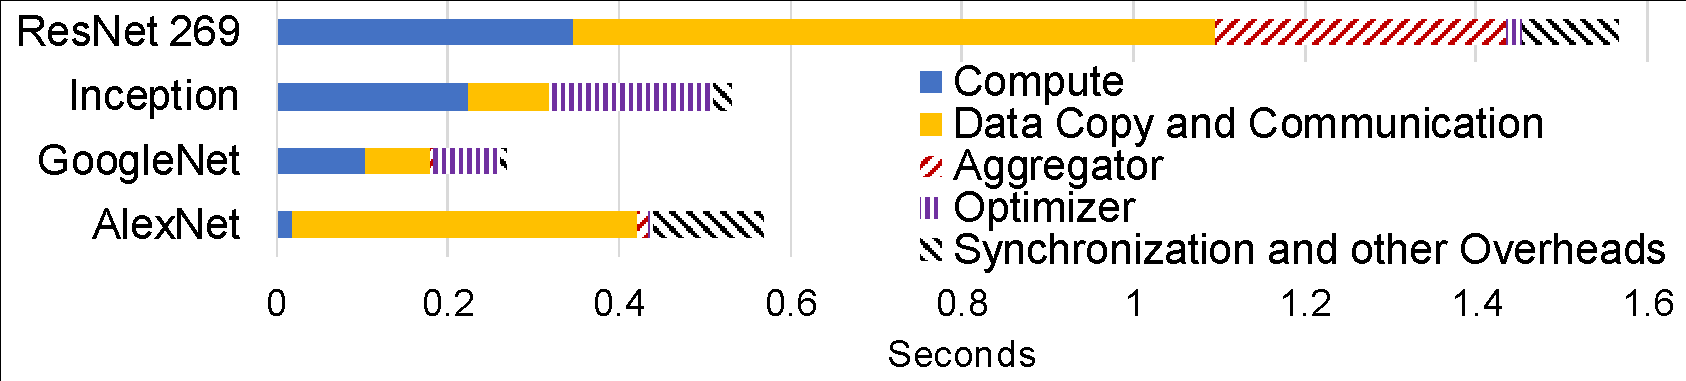
\includegraphics[width=.7\linewidth,trim=3 2 2 4,clip]{Figures/OverheadBreakdown.pdf}
	\caption{Progressive overhead breakdown of different stages during the distributed training pipeline for MxNet distributed training on a 56Gbps network. Link capacity accounts for a small fraction of the copy and communication overhead in this setting.}
	\label{fig:overheadBreakdown}
\end{figure*}

Hardware alone solves only part of the problem. Existing frameworks cannot efficiently use the full hardware capability of \pbox (for example, TensorFlow and MxNet support multiple interfaces only by spawning multiple PS processes). The result is, even with ample communication resources, existing PSs failed to hide communication latency and struggled to scale. Table \ref{table:frameworkPerf} shows that all major DNN training frameworks %failed to achieve 50\% scaling on a 56Gbps IPoIB network (112Gbps bidirectional) in our cluster with 8 workers and PSs. 
do not scale well with a 56 Gbps IPoIB network.

\section{Inefficient Software Stack}

We investigated the cause for MxNet by breaking down the overhead for each major component of a training iteration (legends of Figure \ref{fig:overheadBreakdown}). Since all stages overlap one another, and since ideally we would like early stages to fully hide the latency of later stages, we show \textit{progressive overhead} in Figure \ref{fig:overheadBreakdown}: we gradually turned on different components in the MxNet distributed training pipeline, and each segment shows the \textit{additional overhead that previous stages could not hide}. Specifically, the compute segment shows how long the GPU is active; the data copy segment shows the additional overhead of turning on distributed training without aggregation and optimization; the aggregation and optimization segments show additional overheads of enabling them in that order; and the ``other'' overheads segment includes synchronization and overheads that are not specific to a single component. We explain the overhead for some components:

%\begin{CompactItemize}
	\noindent\textbf{Data copy:} each layer's parameters were copied to and from OS buffers 4 times during parameter exchange.
\vspace{-0.1ex}	

	\noindent \textbf{Aggregation and optimization:} MxNet's approach to achieving parallelism in these operations did not achieve high throughput in our measurements.
\vspace{-0.1ex}	
	
	\noindent \textbf{Synchronization:} MxNet's dispatcher thread needs to synchronize access with ZMQ threads, aggregation threads and an optimization thread via shared queues, leading to bad locality and increased synchronization overhead. 
	
	
\section{\phub Software}
Based on above findings, we propose \phub, an optimized PS implementation that reduces framework overhead with software optimizations. With \phub, we aim to:

% we rearchitected the PS to optimize the network stack, provide efficient gradient aggregation and optimization, and streamline the approach to sending and receiving gradients and model parameters. We also designed \phub to be a rack-scale parameter service, which allows job sharing and topology-aware reduction algorithms.

\begin{enumerate}[noitemsep,topsep=0pt,parsep=0pt,partopsep=0pt]
\item Minimize gradient/model communication overhead.
%\item Gradient data should be laid out to exploit locality and enable overlap.
%\item Preserve locality and enable overlap of gradient processing and receiving.
\item Enable efficient gradient processing and overlap with communication.
\end{enumerate}

We now software optimizations that benefit different stages in distributed training across all common PS configurations. % the network stack optimization, gradient aggregation and optimization, fine-grained key chunking, and chunk-to-core mapping. These software optimizations benefit common PS setups.

\subsection{Network Stack Optimizations}
\label{sec:IBOptimization}
%We sought a solution that enabled zero-copy and kernel bypass for minimal latency and overhead when moving data. 
We sought to mitigate data movement latency with zero-copy and kernel bypass. We chose InfiniBand (IB) since we were already familiar with the Verbs API, and it is available in major cloud providers~\cite{AzureWin5:online}. Note that similar results could be achieved over Ethernet using RoCE, DPDK or other frameworks. We followed the guidelines from~\cite{rdma}; we tried two and one-sided RDMA, and two-sided send/receive operations and found similar performance in our workload. We briefly highlight some implementation details:

\noindent \textbf{Minimal Copy:} Leveraging InfiniBand's zero-copy capability, the only required data copy is between the GPU and main memory. When one GPU is used, this can be eliminated with GPU-Direct RDMA on supported devices.

\noindent \textbf{NUMA-Aware, One-shot Memory Region Registration:} Since a worker can operate on only one model update at a time, it is sufficient to allocate one read buffer (for the current model) and one write buffer (for update reception) for the model. To minimize InfiniBand cache misses, \phub preallocates all buffers in the NUMA domain where the card resides as a contiguous block.

\noindent \textbf{Minimal Metadata:} To maximize bandwidth utilization and minimize parsing overhead, \phub encodes metadata (such as callback ID and message opcode) into InfiniBand's queue pair number and immediate field. This saves \phub an additional PCIe round trip (from IB send scatter/gather) to gather metadata when sending messages.

%\phub leverages InfiniBand's zero-copy ability to reduce copies from the network to  GPU memory by re a per-key aggregation buffer set up during \code{Initialize}; the buffer aggregates gradients from multiple devices before pushing them out to the network. Thus, the only remaining copy to the buffer is from the GPU. For a single GPU, this copy can be eliminated using  GPU-Direct RDMA on supported devices. Before \phub uses InfiniBand as its data plane, it must register all memory used for communication. A worker can have only one model update executing concurrently. Thus, it is sufficient to allocate and register a buffer per worker for gradient reception, and a single buffer for the model. To minimize InfiniBand card memory registration cache misses, \phub pre-allocates all buffers to a single contiguous memory region that it registers. \phub memory registration is NUMA-aware. Memory is allocated on the same NUMA domain where the card resides to reduce QPI traffic between sockets. To keep track of pending operations, some metadata is required, such as current message meaning, sender and receiver information, opcode, and a timestamp used to execute the proper callback. To maximize bandwidth utilization, we encode all metadata into InfiniBand's queue pair number or immediate field. We also designed timestamps to be logical and deterministic, so they can be calculated by combining a global batch number with  message's key. This saves us an additional PCIe round trip (from IB send scatter/gather) to gather metadata when sending messages. 

\subsection{Gradient Aggregation and Optimization}
\label{sec:tallvswide}


% for 2690v4: AVX max speed is 2.1 GHz, 1 256-bit add per cycle (2 if FMA multiplying by 1, but that's annoying)
% so 2.1 GHz * 8-float vectors (32 bits) * (2 reads + 1 write) * 28 cores
% so 470 billion ops/second, 5645 GB/s bidir for 2 read 1 write, 1882 GB/s if aggregation buffers (1read, 1write) are in cache
%% Gradient aggregation could be performed on the CPU or GPU. Here, we posit that the CPU is sufficient for this job.
%% Aggregation is simply vector addition: we read two floats and write one back.
%% For modern CPUs, this is fast: if we keep the processors' AVX ALUs fed, we can perform 470 single-precision giga-adds per second, requiring 5.6TB/s of load/store bandwidth.
%% A typical dual socket server can sustain up to 140GB/s memory bandwidth. 5.6TB/s is impractical for the large vectors involved in DNN training workloads, making aggregation inherently memory bound. There is thus little point in copying gradients to GPU to perform aggregation.
Gradient aggregation could occur in the CPU or GPU~\cite{GeePS}. Here, we posit that the CPU is sufficient for this job.
Aggregation is simply vector addition: we read two floats and write one back.
%Our evaluation hardware is typical of modern dual socket servers. 
With our typical modern dual socket server, if we keep our processors' AVX ALUs fed, we can perform 470 single-precision giga-adds per second, requiring 5.6 TB/s of load/store bandwidth.
But the processors can sustain only 120 GB/s of DRAM bandwidth, making aggregation inherently memory bound. Thus, copying gradients to a GPU for aggregation is not helpful.

\begin{figure}[t!]
    \centering
	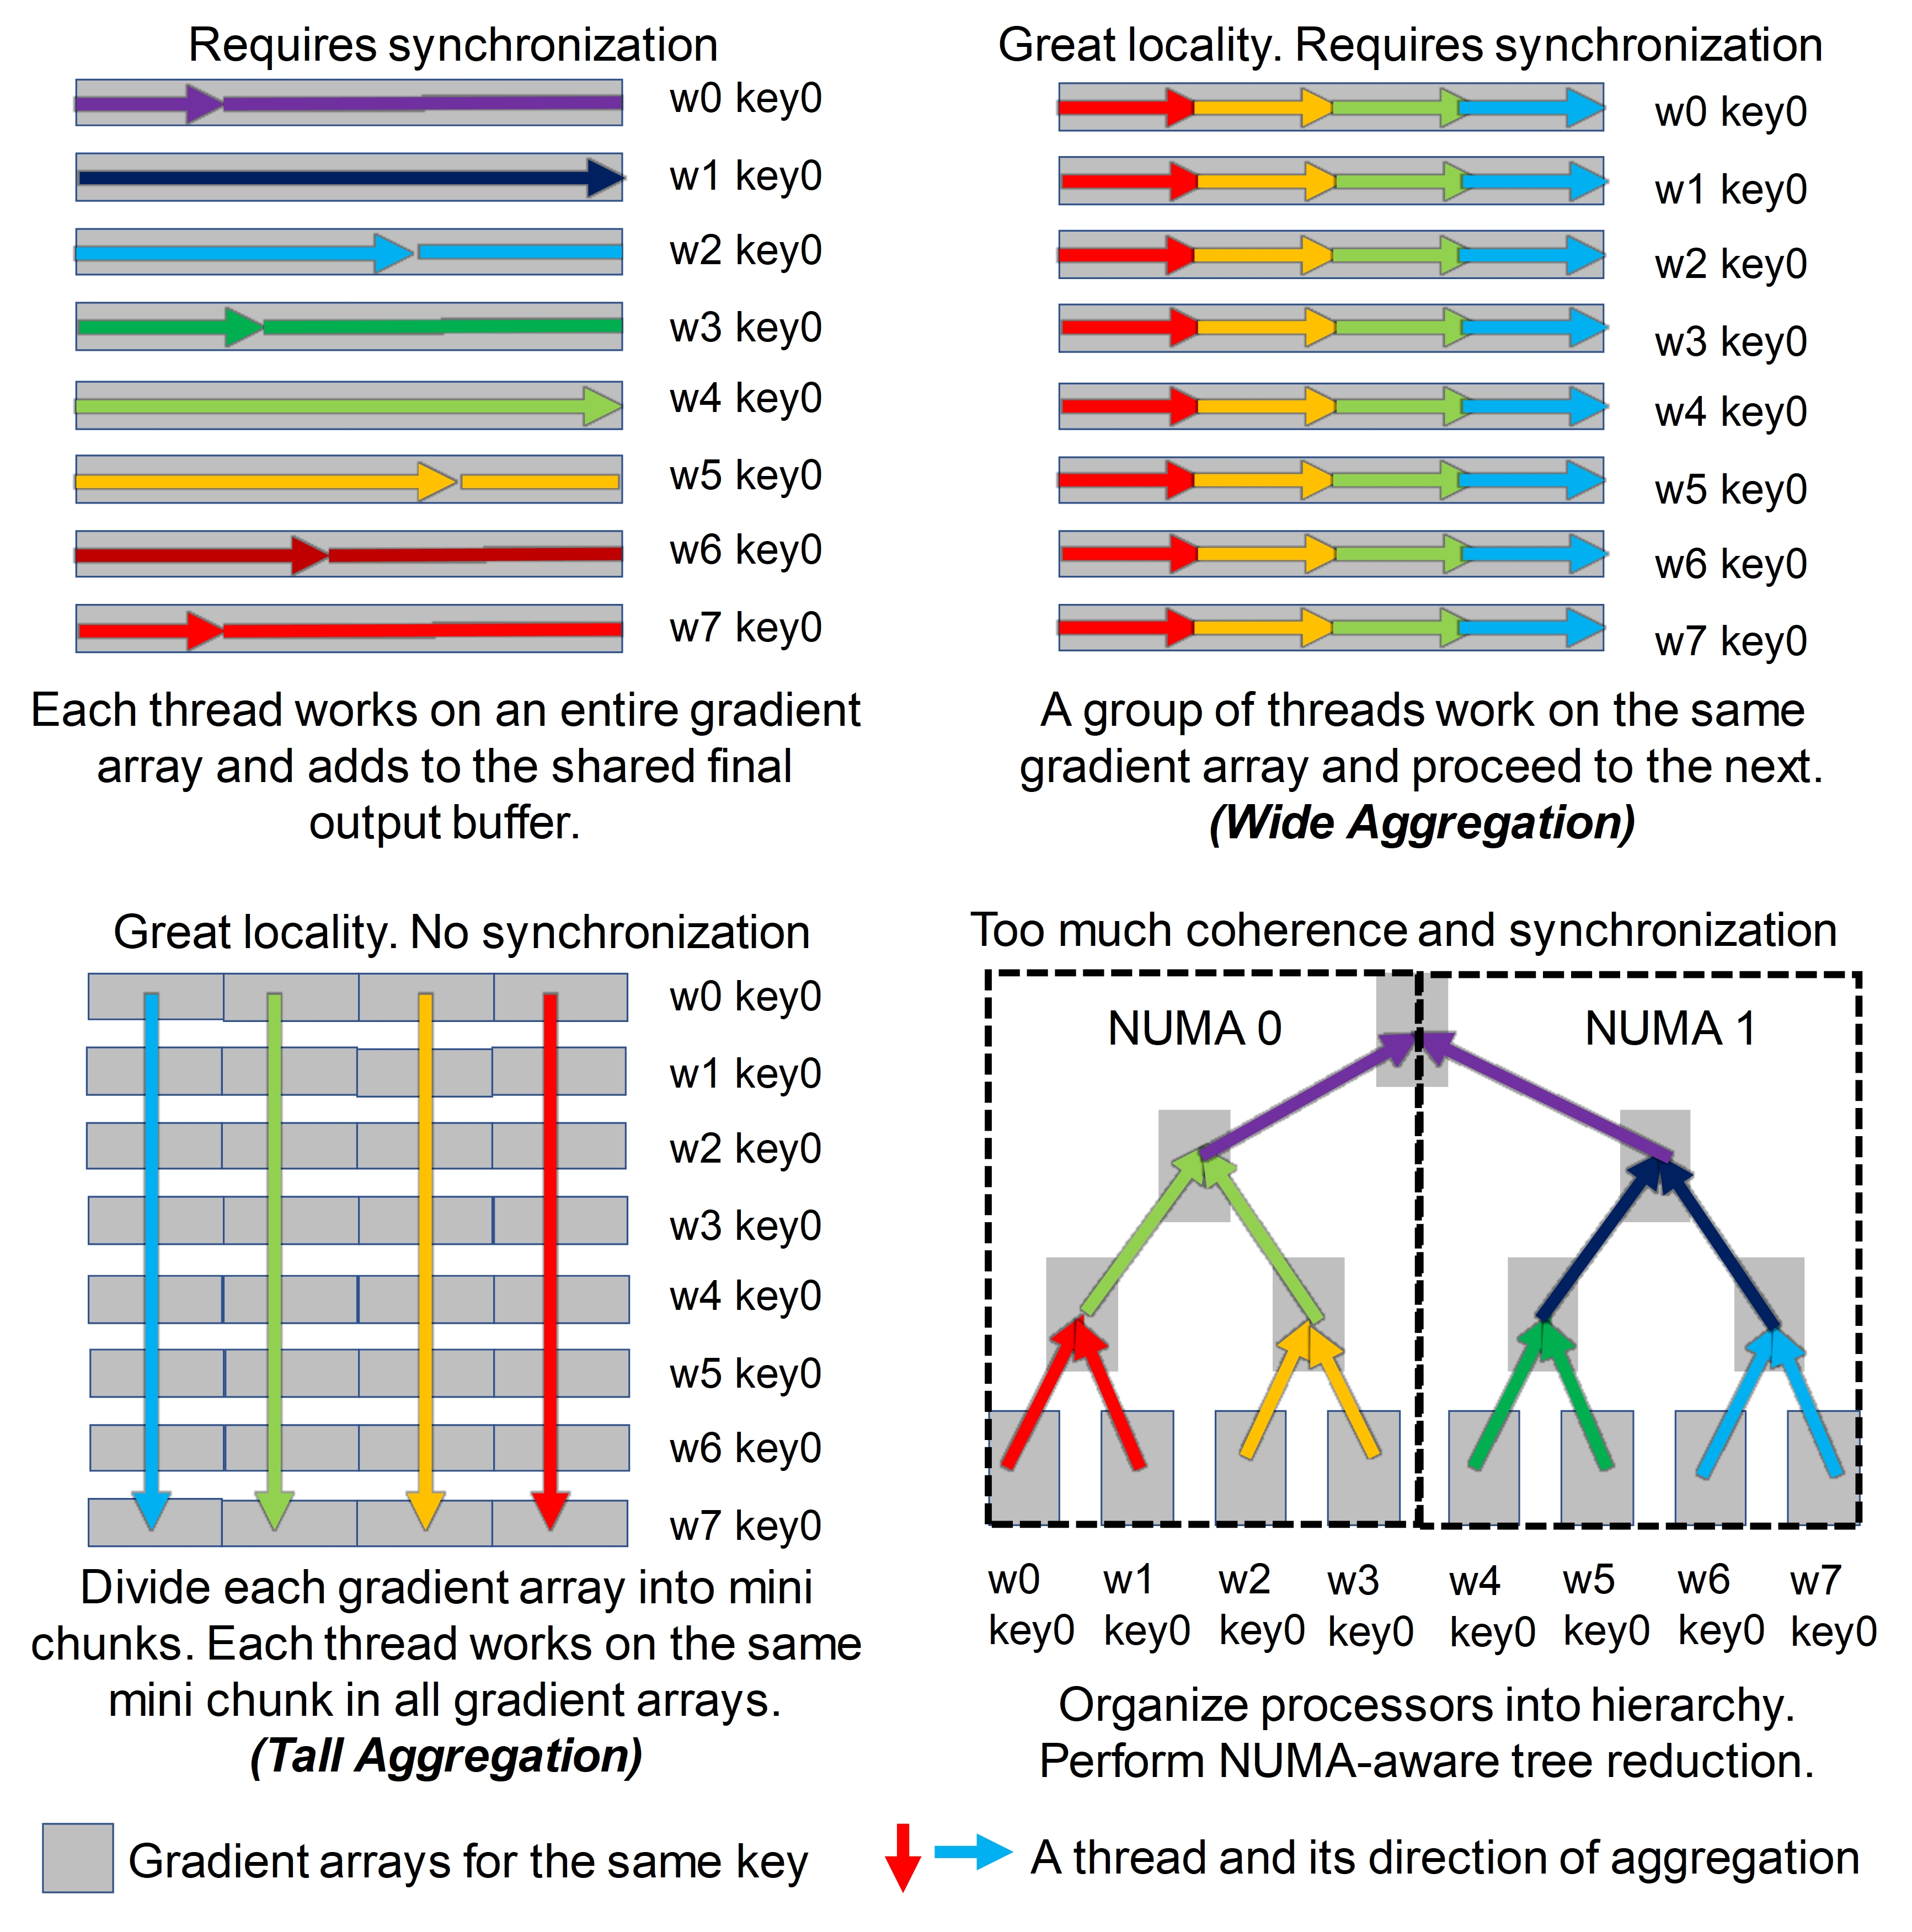
\includegraphics[width=.7\linewidth,trim=5 5 15 5,clip]{Figures/AggregationExperiments.jpg}
	\caption{Ways of gradient aggregation. A thread (arrow) aggregates over the array (gray rectangle) of gradients from a worker. }
	\label{fig:gradientAggregation}
\end{figure}


There are many ways to organize threads to perform aggregation.
%We start with the case where all workers' gradient arrays for a given key are received. 
Figure \ref{fig:gradientAggregation} shows four options we prototyped, assuming gradient arrays are available at once. We found that the best performance was achieved using the two discussed below; other schemes suffered from too much synchronization overhead, poor locality and/or high latency.

\textit{Wide aggregation} is typical to systems like MxNet that call BLAS routines for linear algebra. In these systems, a group of aggregation threads process one gradient array at a time; each thread works on a partition of that array. 
%When the current array is done, the group moves to the next.

A variation of wide aggregation is \textit{tall aggregation}, which chunks a gradient array into mini-chunks of predefined sizes; each thread works independently to process the same chunk across all gradient arrays for a given key. This is the preferable way to organize threads for many reasons.
First, gradient arrays do not arrive instantly. For a large key (e.g., a fully connected layer), aggregation and optimization cannot start for wide aggregation until the key is fully received; for tall aggregation, the process can start as soon as the first chunk is received.
Second, in wide aggregation, it is challenging to balance the number of threads dedicated to aggregation and to optimization, let alone partitioning threads to work on different keys since they can arrive at the same time; %, as the optimal assignment can be DNN dependent; 
thread assignment for tall aggregation is natural.
Third, wide aggregation induces queuing delays: it effectively processes one key at a time versus tall aggregation's many ``mini-queues.''
Fourth, wide aggregation puts many threads to work in lock-step on pieces of data, which incurs non-trivial synchronization overhead; tall aggregation requires no coordination of threads as aggregation is an element-wise operation.

%and tall aggregation allows aggregation to start as soon as a chunk is received, without waiting for the entire gradient array to arrive (some networks have large fully connected layers of size up to tens of megabytes), overlapping communication and computation. More importantly, it is challenging to balance the number of threads that are dedicated to aggregation and optimization if they overlap. 

%Tall aggregation essentially creates many mini queues, alleviating queueing delays. Wide aggregation approach on the other hand, can incur high overhead from repeated thread coordination, and working on only one gradient (which belongs to the same key) at a time effectively forms a queue causing delays. Furthermore, the optimal value for number of threads is workload dependent in wide aggregation. Figure \ref{fig:tallVSWide} compares these two approaches. We chose tall aggregation in \phub.

\phub tracks the number of currently aggregated mini-chunks for a given key. When a chunk is received from all workers, it can be optimized. This step is natural in \phub: the thread that aggregates a particular chunk also optimizes that chunk. As a result, \phub{}'s aggregation and optimization scheme effectively maps a particular chunk to a single core (since \phub pins threads to cores). On the other hand, MxNet uses wide optimization: when a key is fully aggregated, another set of threads is launched to perform aggregation. No overlap occurs between key aggregation and optimization. 
%% \phub tracks the number of currently aggregated chunks for a given key.
%% \phub counts the number of workers for which it has aggregated a chunk.
%% When a chunk has been received from all workers, it can be optimized.
%% This step is natural in \phub: the thread that aggregates a particular chunk also performs optimization for that chunk.
%% As a result, \phub{}'s aggregation and optimization scheme effectively maps a particular chunk to a single core.
%% Conversely, MxNet uses wide optimization: when a key is fully aggregated, a new set of parallel tasks is launched to perform optimization.
%% No overlap occurs between the two steps. Figure \ref{fig:tallVSWide} compares throughput of tall and wide aggregation in \phub and MxNet: tall aggregation/optimization outperforms their wide counterparts.


%Similar to gradient aggregation, optimizer is another element-wise step. \phub naturally assign optimization task of each mini chunk of a key to the core that is responsible for its aggregation (tall optimization). This allows optimization and aggregation of a same key to overlap\footnote{As a side note, MxNet uses wide optimization as well. When a key is fully aggregated, it moves to the optimization stage and potentially another group of threads is launched. There is no overlapping between key aggregation and optimization.}.

%% We implemented two variants of each optimizer: one that uses normal cached loads and stores, and one that bypasses the caches with non-temporal prefetches and stores. This allowed us to test whether caching only the model or gradients wold provide a benefit. We found the temporal version to be more effective. \phub{}'s aggregators and optimizers are fully extensible: implementations that comply with \phub{}'s API can be used during runtime.

We explored the benefits of caching by implementing two variants of each aggregator and optimizer: one using normal cached loads and stores, and one with non-temporal prefetches and stores. We found it beneficial to cache both the model and gradients. \phub{}'s aggregators and optimizers are fully extensible: implementations that comply with \phub{}'s API can be used during runtime.

\subsection{Fine-grained Key Chunking}
%\phub chunks key for two purposes. First, fine-grained key chunking lets \phub balance server and processor core load. This is important because different neural network layers can have significantly different total weight sizes, from a few bytes to tens of MBs. Second, fine-grained key chunking supports tall aggregation and optimization, so processor cores can be fully utilized.

%This makes balancing server and processor core load challenging. By chunking the weight size into a series of virtual layers (a set of virtual keys) of small, fixed size, \phub can balance load of processor cores optimally.These virtual keys are then treated independently in model update; \phub relies on fined grained key chunking to support tall aggregation and optimization, usually at the size of a few to tens of kilobytes.

Chunking in \phub differs from other systems in key ways. Initially, our goal is to balance load at a fine-grained level across cores and interfaces rather than across server shards: chunking is turned on even when a centralized PS is used. Next, we would expect our optimal chunk size to be the smallest message size that can saturate network bandwidth, whereas systems like MxNet prefer larger key chunk sizes to avoid excessive thread synchronization overhead.
%In fact, \phub defaults to 32KB of chunk, while MxNet defaults to a 4MB chunk size.
In fact, \phub's default is 32KB, while MxNet's is 4MB.
Finally, key chunking enables another important optimization: the overlapping of gradient transmission with aggregation and optimization. Aggregation starts only after a key's entire gradient array is received; and for large layers, this adds significant delay. With small key chunks, \phub enables ``streaming'' aggregation and optimization.

\begin{figure}[t!]
	\centering
	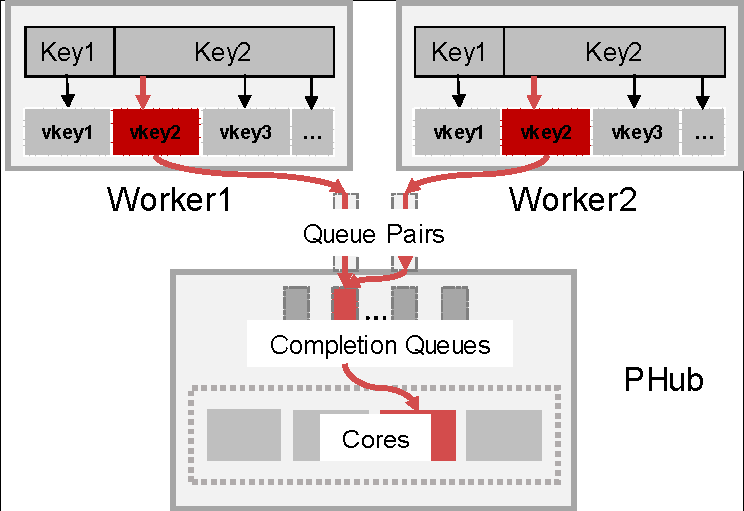
\includegraphics[width=.5\linewidth,trim=1 1 1 1,clip]{Figures/MappingChunkToCore.pdf}
	\caption{The process of mapping a chunk to a core in \phub using fine grained key chunking. Keys are chunked into virtual keys. The highlighted key is delivered to a highlighted (fixed) core through a highlighted (fixed) queue pair and completion queue. }
	\label{fig:mappingChunkToCore}
\end{figure}


\subsection{Mapping a Chunk to a Core}
\label{sec:chunk2core}
\phub's assignment of chunks to cores is computed during initialization. At that time, the set of all keys is sharded across the cores and interfaces available on PS nodes.
A specific chunk is always directed to a particular queue pair,
which is associated with a shared completion queue on the chunk's core.
%the responsible core has a single completion queue for all its associated queue paris.
%which is associated with a completion queue and is eventually processed by that single core.
All message transmission, reception, and processing for that chunk is done on that core. Cores do not synchronize with each other. Once processed, a chunk is transmitted back to the workers on its originating path. The worker side of \phub assembles and disassembles a key, a process that is transparent to the framework.

\phub{}'s chunk assignment scheme provides significant locality benefits. The same key likely arrives around the same time from multiple workers; the associated aggregation buffer is reused during this period. The scheme also encourages locality in the InfiniBand interface in the queue pair and memory registration caches. %, which can further benefit performance.

This scheme imposes challenges in balancing load across cores, queue pairs and completion queues. \phub uses a 4/3 approximation set partition algorithm to balance each component's workload at each level, which produces practically balanced assignments in our experiments. \phub{}'s chunk mapping mechanism is summarized in Figure \ref{fig:mappingChunkToCore}.

\section{The \phub Service API and Interoperability with other Frameworks}
\phub{}'s API is designed for compatibility with multiple DNN training frameworks. Workers use \phub by first calling \code{PHub::CreateService} on the connection manager. This sets up access control and a namespace for the training job and returns a handle. The client side uses the handle to finish setup. \phub uses the namespace and an associated nonce for isolation and access control. 

Jobs call \code{PHub::ConnectService} to rendezvous servers and workers, exchanging addresses for communication. This call replaces \code{Van::Connect} in MxNet, \code{Context::connectFullMesh} in Caffe2 and \code{GrpcServer::Init} in TensorFlow. \code{PHub::InitService} causes the current \phub instance to allocate and register receive and merge buffers. \phub also authenticates each worker's identity using the nonce. Authentication is a one-time overhead and once a connection is established, \phub assumes the remote identity associated with that address/port/queue number does not change during training.

\phub{}'s functional APIs include standard synchronous or asynchronous \code{PHub::Push/Pull} operations that are used in TensorFlow (\code{GraphMgr::SendInputs/RecvOutputs}) and MxNet (\code{KVStoreDist::PushImpl/PullImpl}). \phub also includes a fused \code{PHub::PushPull} operation that perform a push, waits until all pushes are complete, and pulls the latest model. The fused operation often saves a network round-trip as push and pulls are frequently issued consecutively. This operator can serve as a drop-in replacement for Caffe2's \code{Algorithm::Run}.


\section{Interaction of \pbox and \phub}
\phub takes full advantage of \pbox by extending the chunk-to-core mapping scheme%It ensures balance across queue pairs, completion queues, interfaces, cores, and NUMA domains. 
, ensuring balance across interfaces and NUMA domains. \phub further guarantees no inter-processor traffic on \pbox, and completion queues and queue pairs in an interface card are used by only one core in the same NUMA domain to promote locality and avoid coherence traffic. In essence, \pbox forms micro-shards inside a box.

